\scanpage{15}
\mspage{29}

\deleted{radicielle finie (par exemple, soit séparable)}
\inserted{Conditions équivalentes : 1)} \deleted{Pour que} $B$ \deleted{soit}\inserted{est} une
algèbre de Cohen sur $A$ (sous-entendu: pour les topologies habituelles,
-- il faudrait le préciser dans \inserted{4.}7.), \deleted{il f et suffit que}\inserted{2)} $B$
\deleted{soit}\inserted{est} plat sur $A$, complet, et \deleted{que} $B_0=B/\underline{m}B$
\deleted{soit}\inserted{est} une algèbre de Cohen sur $k=A/\underline{m}$, i.e.
formellement simple sur $k$,
\inserted{\unsure{cf} 2.\unsure{6}.}

\deleted{\inserted{3) $B$ est \inserted{complet et} formellement simple sur $A$
\unsure{et satisfait P|et est complet}}}

(On aura noté \deleted{pu} après \inserted{4.}7. que pour une algèbre topologique sur un
corps $k$, Cohen = adique et formellement simple ). \deleted{La nécessité}
\inserted{$1)\Longrightarrow2)$ \deleted{\unsure{est}}} étant
déjà acquis\deleted{e} (sans hypothèse de multiplicité radicielle finie), prouvons
\deleted{la suffisance}\inserted{$2)\Longrightarrow1)$}. En vertu de la définition, on est ramené simplement à
prouver que $B$ satisfait la condition P. Cela nous ramène au cas où $A$ est
artinien. En vertu du N°2, on sait que $B_0$ est régulier, considérons un
système régulier de paramètres de $B_0$ (un système de paramètres formant
une $B_0$-suite suffirait), relevons le en un système de paramètres de $B$,
soit $x=(x_1,\ldots,x_r)$. Alors les idéaux engendrés par les $x^n=(x_1^n,\ldots,x_r^n)$,
pour $n\geq0$, forment un système fondamental de voisinages\inserted{$I_n$} de 0 dans
$B$, d'autre part on constate aussitôt que les $B/J_n$ sont des modules
plats sur $A$ (il y a un \deleted{lemme} corollaire dans la platitude supérieure,
dans le cas où on divise par un seul élément \deleted{non divi} régulier, cas
auquel on est ramené aussitôt). Comme $A$ est artinien, ils sont donc
projectifs. \deleted{\unsure{cqfd.}}

\deleted{\unsure{Enfin,} \illegible{2} \unsure{que} $3)\Longrightarrow2)$ \illegible{2}
\unsure{3.8.}}
\deleted{\unsure{d'après} 2) d')}
\inserted{en utilisant le th. d'existence ci-dessous 3.9.}

\deleted{NB On n'a utilisé l'hypothèse sur la multiplicité radicielle que
pour \deleted{pouvoir} savoir que $B_0$ est Cohen-Macaulay.}
\deleted{L'hypothèse faite est
très probablement inutile. Serre vient de me dire que Mac-Lane a prouvé
la réciproque de 2.3. sans hypothèse de multiplicité rad finie, dans
``Note on a relative structure of p-adic fields'' Ann Math t 41 1940,
page 751 --753. Cela vaudrait peut-être le coup, pour \deleted{liquider d} le coup
d'oeuil, que tu regardes cela et donnes le résultat complet dans 2.3. On}

\margin{\figure{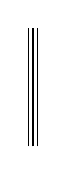
\begin{tikzpicture}\draw (0,0)--(0,1.5);\draw (.06,0)--(.06,1.5);\draw (.12,0)--(.12,1.5);\end{tikzpicture}}}
\mspage{14}
